\section{Simple, Naïve Algorithm}
This is the simple, straightforward, naïve implementation we did before any smart ideas and optimizations.
\subsection{Algorithm Description}
The Naïve Wavelet Tree construction algorithm is recursively defined, calling itself to construct the left and right sub-tree from the root node and down. At each recursion the algorithm splits the given alphabet in two halves and traverses the given string putting each character into a left or right partition based on whether the character was in the left or right half of the alphabet.

\begin{mdframed}[nobreak]
\begin{algorithmic}
\Function {ConstructNode} {$String, Alphabet$}
\If{$Alphabet.Size() = 1$ or $String.Length() = 0$}
	\State \Return
\EndIf
\State Split $Alphabet$ into $LeftAlphabet$ and $RightAlphabet$
\State $Split \gets$ middle character in $Alphabet$
\ForAll {$Character$ in $String$}
	\If {$Character < Split$}
		\State $LeftString.Append(Character)$
		\State $Bitmap.Append(0)$
	\Else
		\State $RightString.Append(Character)$
		\State $Bitmap.Append(1)$
	\EndIf
\EndFor
\State $LeftNode \gets$ \Call {ConstructNode} {$LeftAlphabet, LeftString$}
\State $RightNode \gets$ \Call {ConstructNode} {$RightAlphabet, RightString$}
\EndFunction

\State \Call {ConstructNode} {InputString, InputAlphabet}
\end{algorithmic}
\end{mdframed}

\noindent In our implementation, $Alphabet$, $LeftAlphabet$, and $RightAlphabet$ are stored as two integer values each: a minimum and a maximum. It is explained in~\ref{sec:UsingIntAsChar} how this is equivalent to storing the full alphabet and passing pointers into it around. $Bitmap$ is stored as a \texttt{vector<bool>} which is tightly packed, only using 1 bit per bool\footnote{\url{http://www.cplusplus.com/reference/vector/vector-bool/}}.

\subsection{Optimizations}
\subsubsection{Binary Rank using Popcount}
\label{sec:popcountBinaryRank}
Binary Rank was first implemented using the algorithm described in \ref{sec:TheoryBinaryRank}. 
To improve on this, we found the intrinsic cpu instruction \texttt{popcount} which will count the number of 1s in the binary representation of the number we pass to it.
We can get an \texttt{unsigned long} pointer from the \texttt{vector<bool>} bitmap into the backing array. We will therefore be working on \texttt{unsigned long}s and call their size (64 bits on machine 1) our wordsize.
When using \texttt{popcount}, \textproc{BinaryRank} remains in theory an $O(N/wordsize) = O(N)$ operation, as \textit{wordsize} is a constant factor, but it has a large practical effect on performance as can be seen in section~\ref{sec:experimentPopcountRankSelect}.

To use \texttt{popcount} we call \texttt{\_\_builtin\_popcountl} which is a function built into the GCC compiler \citep{Popcount-GCC-Builtin}. 
It takes an \texttt{unsigned long} as a parameter and returns the number of 1s in it. \texttt{\_\_builtin\_popcountl} will automatically figure out how to do popcount based on what CPU you are using. Popcount as an intrinsic cpu instruction is supported on both AMD \citep{AMD-Popcount} and Intel arhitectures \citep{Intel-Popcount}.
We have verified, by looking at the produced assembly code, that \texttt{popcount} is calculated using a cpu instruction \texttt{popcnt} on our computers which we assume to be the fastest way to calculate \texttt{popcount} since it is only a single instruction.
	
The binary rank can then be found by summing the result of calling \texttt{popcount} on each word of the bitmap up to a given \textit{position}.
When the position argument of the rank query is not a multiple of the word size, we need to constrain what part of the last word is counted using \texttt{popcount}. This can be done by constructing a bitmask by bitshifting the number 1 \textit{position} times towards the most significant bit and then subtracting one, as that will create a word where the \textit{position} least significant bits are set to 1 and the rest to 0.
Then we do a bitwise \texttt{AND} operation of this bitmask and the word containing the bit corresponding to \textit{position}, and call \texttt{popcount} on the result. 

As also noted in~\citep{Navjda13}, we don't need to count the number of 0s, although required by the algorithm, as we can simply take the number of bits in the string and subtract the number of 1s to calculate the number of 0s.

\subsubsection{Binary Select using Popcount}
\label{sec:ImplBinarySelect}
We improved \textproc{Binary Select} by again using the \texttt{popcount} instruction. 
We iterate through the words of the bitmap and call \texttt{popcount} for each word and sum up the results along the way. 
When the sum after the next word would be greater than the sought number of occurrences we discard the \texttt{popcount} result for the next word and fall back to the simple binary select for that next word to find the position within that word.

Defining the input occurrence parameter as $io$, the number of words iterated through so far $w$, the sum so far $sum$, and the wordsize $ws$, the occurrence argument for that last simple binary select is then the $io - sum$ and the output position is $w \times ws + \textproc{SimpleBinaryRank}(bitmapwords[ws+1], io - sum)$.

Again, when popcount for 0s instead of 1s is needed, we simply subtract the result of \texttt{popcount} from 1 to obtain the count of 0s.

\subsection{Experiments}

\subsubsection{Running time of Tree Construction vs Alphabet Size}
Looks like it's branch mispredictions...
\begin{figure}
	\caption{Wall Time and Branch Mispredictions}
	\begin{subfigure}{\textwidth}
		% GNUPLOT: LaTeX picture with Postscript
\begingroup
  \makeatletter
  \providecommand\color[2][]{%
    \GenericError{(gnuplot) \space\space\space\@spaces}{%
      Package color not loaded in conjunction with
      terminal option `colourtext'%
    }{See the gnuplot documentation for explanation.%
    }{Either use 'blacktext' in gnuplot or load the package
      color.sty in LaTeX.}%
    \renewcommand\color[2][]{}%
  }%
  \providecommand\includegraphics[2][]{%
    \GenericError{(gnuplot) \space\space\space\@spaces}{%
      Package graphicx or graphics not loaded%
    }{See the gnuplot documentation for explanation.%
    }{The gnuplot epslatex terminal needs graphicx.sty or graphics.sty.}%
    \renewcommand\includegraphics[2][]{}%
  }%
  \providecommand\rotatebox[2]{#2}%
  \@ifundefined{ifGPcolor}{%
    \newif\ifGPcolor
    \GPcolortrue
  }{}%
  \@ifundefined{ifGPblacktext}{%
    \newif\ifGPblacktext
    \GPblacktexttrue
  }{}%
  % define a \g@addto@macro without @ in the name:
  \let\gplgaddtomacro\g@addto@macro
  % define empty templates for all commands taking text:
  \gdef\gplbacktext{}%
  \gdef\gplfronttext{}%
  \makeatother
  \ifGPblacktext
    % no textcolor at all
    \def\colorrgb#1{}%
    \def\colorgray#1{}%
  \else
    % gray or color?
    \ifGPcolor
      \def\colorrgb#1{\color[rgb]{#1}}%
      \def\colorgray#1{\color[gray]{#1}}%
      \expandafter\def\csname LTw\endcsname{\color{white}}%
      \expandafter\def\csname LTb\endcsname{\color{black}}%
      \expandafter\def\csname LTa\endcsname{\color{black}}%
      \expandafter\def\csname LT0\endcsname{\color[rgb]{1,0,0}}%
      \expandafter\def\csname LT1\endcsname{\color[rgb]{0,1,0}}%
      \expandafter\def\csname LT2\endcsname{\color[rgb]{0,0,1}}%
      \expandafter\def\csname LT3\endcsname{\color[rgb]{1,0,1}}%
      \expandafter\def\csname LT4\endcsname{\color[rgb]{0,1,1}}%
      \expandafter\def\csname LT5\endcsname{\color[rgb]{1,1,0}}%
      \expandafter\def\csname LT6\endcsname{\color[rgb]{0,0,0}}%
      \expandafter\def\csname LT7\endcsname{\color[rgb]{1,0.3,0}}%
      \expandafter\def\csname LT8\endcsname{\color[rgb]{0.5,0.5,0.5}}%
    \else
      % gray
      \def\colorrgb#1{\color{black}}%
      \def\colorgray#1{\color[gray]{#1}}%
      \expandafter\def\csname LTw\endcsname{\color{white}}%
      \expandafter\def\csname LTb\endcsname{\color{black}}%
      \expandafter\def\csname LTa\endcsname{\color{black}}%
      \expandafter\def\csname LT0\endcsname{\color{black}}%
      \expandafter\def\csname LT1\endcsname{\color{black}}%
      \expandafter\def\csname LT2\endcsname{\color{black}}%
      \expandafter\def\csname LT3\endcsname{\color{black}}%
      \expandafter\def\csname LT4\endcsname{\color{black}}%
      \expandafter\def\csname LT5\endcsname{\color{black}}%
      \expandafter\def\csname LT6\endcsname{\color{black}}%
      \expandafter\def\csname LT7\endcsname{\color{black}}%
      \expandafter\def\csname LT8\endcsname{\color{black}}%
    \fi
  \fi
  \setlength{\unitlength}{0.0500bp}%
  \begin{picture}(7920.00,4752.00)%
    \gplgaddtomacro\gplbacktext{%
      \csname LTb\endcsname%
      \put(1210,704){\makebox(0,0)[r]{\strut{} 0}}%
      \put(1210,1461){\makebox(0,0)[r]{\strut{} 0.005}}%
      \put(1210,2217){\makebox(0,0)[r]{\strut{} 0.01}}%
      \put(1210,2974){\makebox(0,0)[r]{\strut{} 0.015}}%
      \put(1210,3730){\makebox(0,0)[r]{\strut{} 0.02}}%
      \put(1210,4487){\makebox(0,0)[r]{\strut{} 0.025}}%
      \put(1342,484){\makebox(0,0){\strut{}$2^{6}$}}%
      \put(2225,484){\makebox(0,0){\strut{}$2^{8}$}}%
      \put(3108,484){\makebox(0,0){\strut{}$2^{10}$}}%
      \put(3991,484){\makebox(0,0){\strut{}$2^{12}$}}%
      \put(4874,484){\makebox(0,0){\strut{}$2^{14}$}}%
      \put(5757,484){\makebox(0,0){\strut{}$2^{16}$}}%
      \put(6640,484){\makebox(0,0){\strut{}$2^{18}$}}%
      \put(7523,484){\makebox(0,0){\strut{}$2^{20}$}}%
      \put(176,2595){\rotatebox{-270}{\makebox(0,0){\strut{}Wall Time (microsec)}}}%
      \put(4432,154){\makebox(0,0){\strut{}Alphabet Size \small (log scale)}}%
    }%
    \gplgaddtomacro\gplfronttext{%
      \csname LTb\endcsname%
      \put(6536,4204){\makebox(0,0)[r]{\strut{}\large $\frac{Wall Time}{10^7 \cdot log(\sigma)}$}}%
    }%
    \gplbacktext
    \put(0,0){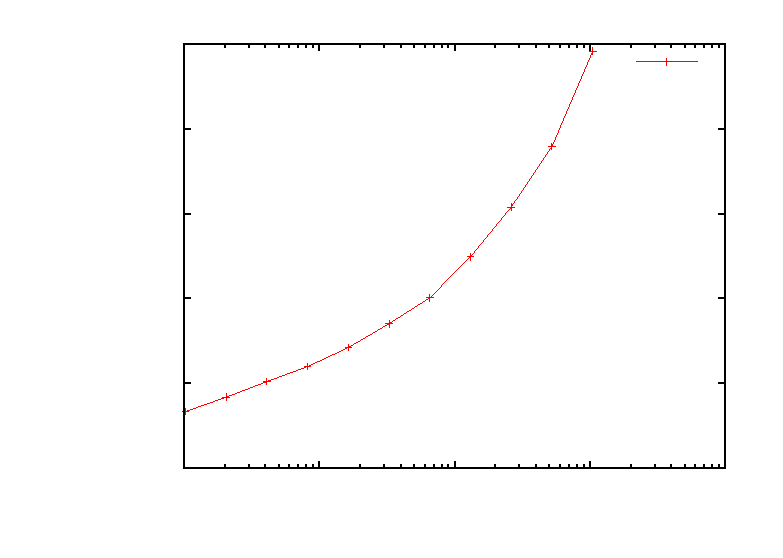
\includegraphics{naiveIntegerAlphabetSize_WallTime}}%
    \gplfronttext
  \end{picture}%
\endgroup

		\caption{Wall Time}
	\end{subfigure}
	
	\begin{subfigure}{\textwidth}
		% GNUPLOT: LaTeX picture with Postscript
\begingroup
  \makeatletter
  \providecommand\color[2][]{%
    \GenericError{(gnuplot) \space\space\space\@spaces}{%
      Package color not loaded in conjunction with
      terminal option `colourtext'%
    }{See the gnuplot documentation for explanation.%
    }{Either use 'blacktext' in gnuplot or load the package
      color.sty in LaTeX.}%
    \renewcommand\color[2][]{}%
  }%
  \providecommand\includegraphics[2][]{%
    \GenericError{(gnuplot) \space\space\space\@spaces}{%
      Package graphicx or graphics not loaded%
    }{See the gnuplot documentation for explanation.%
    }{The gnuplot epslatex terminal needs graphicx.sty or graphics.sty.}%
    \renewcommand\includegraphics[2][]{}%
  }%
  \providecommand\rotatebox[2]{#2}%
  \@ifundefined{ifGPcolor}{%
    \newif\ifGPcolor
    \GPcolortrue
  }{}%
  \@ifundefined{ifGPblacktext}{%
    \newif\ifGPblacktext
    \GPblacktexttrue
  }{}%
  % define a \g@addto@macro without @ in the name:
  \let\gplgaddtomacro\g@addto@macro
  % define empty templates for all commands taking text:
  \gdef\gplbacktext{}%
  \gdef\gplfronttext{}%
  \makeatother
  \ifGPblacktext
    % no textcolor at all
    \def\colorrgb#1{}%
    \def\colorgray#1{}%
  \else
    % gray or color?
    \ifGPcolor
      \def\colorrgb#1{\color[rgb]{#1}}%
      \def\colorgray#1{\color[gray]{#1}}%
      \expandafter\def\csname LTw\endcsname{\color{white}}%
      \expandafter\def\csname LTb\endcsname{\color{black}}%
      \expandafter\def\csname LTa\endcsname{\color{black}}%
      \expandafter\def\csname LT0\endcsname{\color[rgb]{1,0,0}}%
      \expandafter\def\csname LT1\endcsname{\color[rgb]{0,1,0}}%
      \expandafter\def\csname LT2\endcsname{\color[rgb]{0,0,1}}%
      \expandafter\def\csname LT3\endcsname{\color[rgb]{1,0,1}}%
      \expandafter\def\csname LT4\endcsname{\color[rgb]{0,1,1}}%
      \expandafter\def\csname LT5\endcsname{\color[rgb]{1,1,0}}%
      \expandafter\def\csname LT6\endcsname{\color[rgb]{0,0,0}}%
      \expandafter\def\csname LT7\endcsname{\color[rgb]{1,0.3,0}}%
      \expandafter\def\csname LT8\endcsname{\color[rgb]{0.5,0.5,0.5}}%
    \else
      % gray
      \def\colorrgb#1{\color{black}}%
      \def\colorgray#1{\color[gray]{#1}}%
      \expandafter\def\csname LTw\endcsname{\color{white}}%
      \expandafter\def\csname LTb\endcsname{\color{black}}%
      \expandafter\def\csname LTa\endcsname{\color{black}}%
      \expandafter\def\csname LT0\endcsname{\color{black}}%
      \expandafter\def\csname LT1\endcsname{\color{black}}%
      \expandafter\def\csname LT2\endcsname{\color{black}}%
      \expandafter\def\csname LT3\endcsname{\color{black}}%
      \expandafter\def\csname LT4\endcsname{\color{black}}%
      \expandafter\def\csname LT5\endcsname{\color{black}}%
      \expandafter\def\csname LT6\endcsname{\color{black}}%
      \expandafter\def\csname LT7\endcsname{\color{black}}%
      \expandafter\def\csname LT8\endcsname{\color{black}}%
    \fi
  \fi
  \setlength{\unitlength}{0.0500bp}%
  \begin{picture}(7200.00,5040.00)%
    \gplgaddtomacro\gplbacktext{%
      \csname LTb\endcsname%
      \put(1474,704){\makebox(0,0)[r]{\strut{} 4e+07}}%
      \put(1474,1286){\makebox(0,0)[r]{\strut{} 6e+07}}%
      \put(1474,1867){\makebox(0,0)[r]{\strut{} 8e+07}}%
      \put(1474,2449){\makebox(0,0)[r]{\strut{} 1e+08}}%
      \put(1474,3030){\makebox(0,0)[r]{\strut{} 1.2e+08}}%
      \put(1474,3612){\makebox(0,0)[r]{\strut{} 1.4e+08}}%
      \put(1474,4193){\makebox(0,0)[r]{\strut{} 1.6e+08}}%
      \put(1474,4775){\makebox(0,0)[r]{\strut{} 1.8e+08}}%
      \put(1606,484){\makebox(0,0){\strut{} 1000}}%
      \put(2905,484){\makebox(0,0){\strut{} 10000}}%
      \put(4205,484){\makebox(0,0){\strut{} 100000}}%
      \put(5504,484){\makebox(0,0){\strut{} 1e+06}}%
      \put(6803,484){\makebox(0,0){\strut{} 1e+07}}%
      \put(176,2739){\rotatebox{-270}{\makebox(0,0){\strut{}Wall Time (microsec)}}}%
      \put(4204,154){\makebox(0,0){\strut{}Alphabet Size \small (log scale)}}%
    }%
    \gplgaddtomacro\gplfronttext{%
      \csname LTb\endcsname%
      \put(5816,4602){\makebox(0,0)[r]{\strut{}Branch Miss}}%
    }%
    \gplbacktext
    \put(0,0){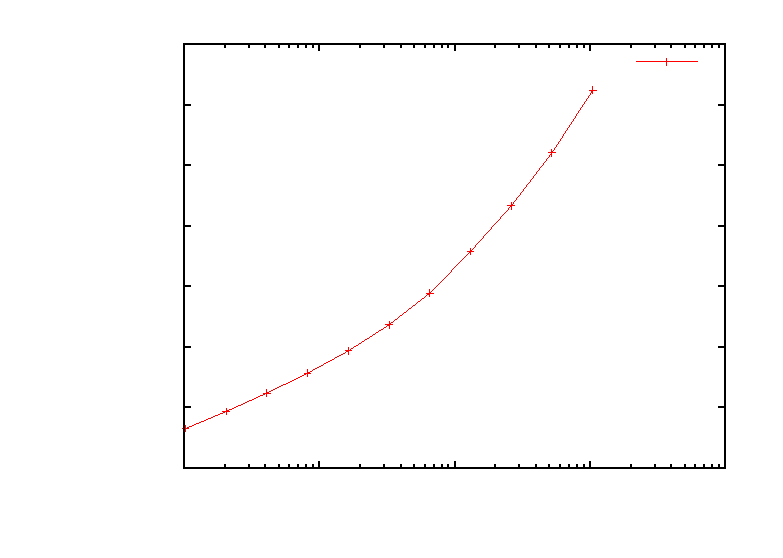
\includegraphics{naiveIntegerAlphabetSize_BM}}%
    \gplfronttext
  \end{picture}%
\endgroup

		\caption{Branch Mispredictions}
	\end{subfigure}
\end{figure}

\begin{figure}
	% GNUPLOT: LaTeX picture with Postscript
\begingroup
  \makeatletter
  \providecommand\color[2][]{%
    \GenericError{(gnuplot) \space\space\space\@spaces}{%
      Package color not loaded in conjunction with
      terminal option `colourtext'%
    }{See the gnuplot documentation for explanation.%
    }{Either use 'blacktext' in gnuplot or load the package
      color.sty in LaTeX.}%
    \renewcommand\color[2][]{}%
  }%
  \providecommand\includegraphics[2][]{%
    \GenericError{(gnuplot) \space\space\space\@spaces}{%
      Package graphicx or graphics not loaded%
    }{See the gnuplot documentation for explanation.%
    }{The gnuplot epslatex terminal needs graphicx.sty or graphics.sty.}%
    \renewcommand\includegraphics[2][]{}%
  }%
  \providecommand\rotatebox[2]{#2}%
  \@ifundefined{ifGPcolor}{%
    \newif\ifGPcolor
    \GPcolortrue
  }{}%
  \@ifundefined{ifGPblacktext}{%
    \newif\ifGPblacktext
    \GPblacktexttrue
  }{}%
  % define a \g@addto@macro without @ in the name:
  \let\gplgaddtomacro\g@addto@macro
  % define empty templates for all commands taking text:
  \gdef\gplbacktext{}%
  \gdef\gplfronttext{}%
  \makeatother
  \ifGPblacktext
    % no textcolor at all
    \def\colorrgb#1{}%
    \def\colorgray#1{}%
  \else
    % gray or color?
    \ifGPcolor
      \def\colorrgb#1{\color[rgb]{#1}}%
      \def\colorgray#1{\color[gray]{#1}}%
      \expandafter\def\csname LTw\endcsname{\color{white}}%
      \expandafter\def\csname LTb\endcsname{\color{black}}%
      \expandafter\def\csname LTa\endcsname{\color{black}}%
      \expandafter\def\csname LT0\endcsname{\color[rgb]{1,0,0}}%
      \expandafter\def\csname LT1\endcsname{\color[rgb]{0,1,0}}%
      \expandafter\def\csname LT2\endcsname{\color[rgb]{0,0,1}}%
      \expandafter\def\csname LT3\endcsname{\color[rgb]{1,0,1}}%
      \expandafter\def\csname LT4\endcsname{\color[rgb]{0,1,1}}%
      \expandafter\def\csname LT5\endcsname{\color[rgb]{1,1,0}}%
      \expandafter\def\csname LT6\endcsname{\color[rgb]{0,0,0}}%
      \expandafter\def\csname LT7\endcsname{\color[rgb]{1,0.3,0}}%
      \expandafter\def\csname LT8\endcsname{\color[rgb]{0.5,0.5,0.5}}%
    \else
      % gray
      \def\colorrgb#1{\color{black}}%
      \def\colorgray#1{\color[gray]{#1}}%
      \expandafter\def\csname LTw\endcsname{\color{white}}%
      \expandafter\def\csname LTb\endcsname{\color{black}}%
      \expandafter\def\csname LTa\endcsname{\color{black}}%
      \expandafter\def\csname LT0\endcsname{\color{black}}%
      \expandafter\def\csname LT1\endcsname{\color{black}}%
      \expandafter\def\csname LT2\endcsname{\color{black}}%
      \expandafter\def\csname LT3\endcsname{\color{black}}%
      \expandafter\def\csname LT4\endcsname{\color{black}}%
      \expandafter\def\csname LT5\endcsname{\color{black}}%
      \expandafter\def\csname LT6\endcsname{\color{black}}%
      \expandafter\def\csname LT7\endcsname{\color{black}}%
      \expandafter\def\csname LT8\endcsname{\color{black}}%
    \fi
  \fi
  \setlength{\unitlength}{0.0500bp}%
  \begin{picture}(7200.00,5040.00)%
    \gplgaddtomacro\gplbacktext{%
      \csname LTb\endcsname%
      \put(1474,704){\makebox(0,0)[r]{\strut{} 0}}%
      \put(1474,1156){\makebox(0,0)[r]{\strut{} 5e+06}}%
      \put(1474,1609){\makebox(0,0)[r]{\strut{} 1e+07}}%
      \put(1474,2061){\makebox(0,0)[r]{\strut{} 1.5e+07}}%
      \put(1474,2513){\makebox(0,0)[r]{\strut{} 2e+07}}%
      \put(1474,2966){\makebox(0,0)[r]{\strut{} 2.5e+07}}%
      \put(1474,3418){\makebox(0,0)[r]{\strut{} 3e+07}}%
      \put(1474,3870){\makebox(0,0)[r]{\strut{} 3.5e+07}}%
      \put(1474,4323){\makebox(0,0)[r]{\strut{} 4e+07}}%
      \put(1474,4775){\makebox(0,0)[r]{\strut{} 4.5e+07}}%
      \put(1606,484){\makebox(0,0){\strut{} 1000}}%
      \put(2905,484){\makebox(0,0){\strut{} 10000}}%
      \put(4205,484){\makebox(0,0){\strut{} 100000}}%
      \put(5504,484){\makebox(0,0){\strut{} 1e+06}}%
      \put(6803,484){\makebox(0,0){\strut{} 1e+07}}%
      \put(176,2739){\rotatebox{-270}{\makebox(0,0){\strut{}Amount}}}%
      \put(4204,154){\makebox(0,0){\strut{}Alphabet Size \small (log scale)}}%
    }%
    \gplgaddtomacro\gplfronttext{%
      \csname LTb\endcsname%
      \put(5816,4602){\makebox(0,0)[r]{\strut{}TLB Miss}}%
      \csname LTb\endcsname%
      \put(5816,4382){\makebox(0,0)[r]{\strut{}L1 CM}}%
      \csname LTb\endcsname%
      \put(5816,4162){\makebox(0,0)[r]{\strut{}L2 CM}}%
      \csname LTb\endcsname%
      \put(5816,3942){\makebox(0,0)[r]{\strut{}L3 CM}}%
    }%
    \gplbacktext
    \put(0,0){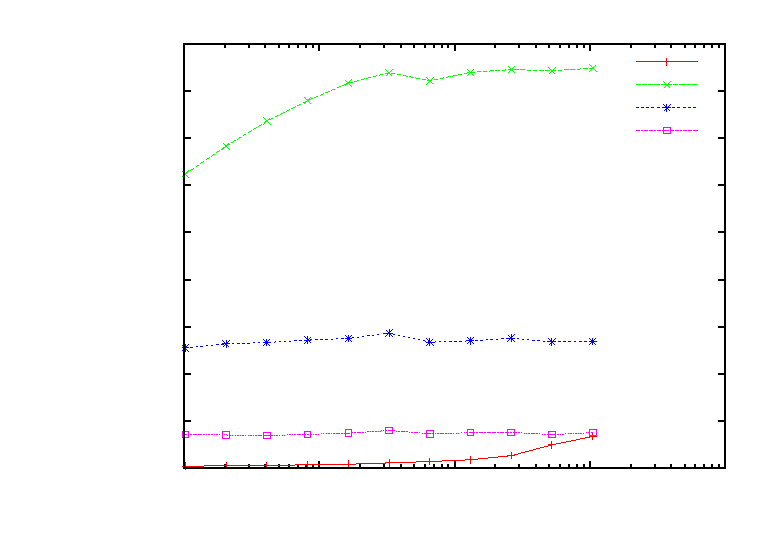
\includegraphics{naiveIntegerAlphabetSize_TLB_CM}}%
    \gplfronttext
  \end{picture}%
\endgroup

	\caption{Translation Lookaside Buffer Misses, and Level 1-3 Cache Misses}
\end{figure}


\subsubsection{Rank and Select using Popcount}
\label{sec:experimentPopcountRankSelect}
We wanted to see how much of an improvement using the native cpu instruction \texttt{popcount} was, and how it affected the cache misses, branch mispredictions and TLB misses.

We wrote our program to build the tree, then run 100 rank or select queries for characters evenly distributed across the alphabet.
For the rank queries we used the size of the input string as the positional argument so that the entire tree would be used in the query.
We ran each test 5 times and used the average value for each measurement.
For the select queries we queried for the 2000th occurrence because previously run rank queries showed us that each character we queried for occurred about 2400-2600 times in the input string we used, and we could then be reasonably sure that each character in the alphabet would occur at least 2000 times.

By querying for characters evenly distributed along the alphabet, we ensure that the queries together traverse most of the tree, and thus try to avoid having everything cached for every query. Another option would have been to use randomly selected characters, but that would have introduced some uncertainty as to whether it was the access pattern or the change in algorithm that caused a difference in running time.



\begin{figure}
\caption{Simple Binary Rank vs. Binary Rank using the Popcount instruction.}
\label{fig:rankPopcountDiff}
% GNUPLOT: LaTeX picture with Postscript
\begingroup
  \makeatletter
  \providecommand\color[2][]{%
    \GenericError{(gnuplot) \space\space\space\@spaces}{%
      Package color not loaded in conjunction with
      terminal option `colourtext'%
    }{See the gnuplot documentation for explanation.%
    }{Either use 'blacktext' in gnuplot or load the package
      color.sty in LaTeX.}%
    \renewcommand\color[2][]{}%
  }%
  \providecommand\includegraphics[2][]{%
    \GenericError{(gnuplot) \space\space\space\@spaces}{%
      Package graphicx or graphics not loaded%
    }{See the gnuplot documentation for explanation.%
    }{The gnuplot epslatex terminal needs graphicx.sty or graphics.sty.}%
    \renewcommand\includegraphics[2][]{}%
  }%
  \providecommand\rotatebox[2]{#2}%
  \@ifundefined{ifGPcolor}{%
    \newif\ifGPcolor
    \GPcolortrue
  }{}%
  \@ifundefined{ifGPblacktext}{%
    \newif\ifGPblacktext
    \GPblacktexttrue
  }{}%
  % define a \g@addto@macro without @ in the name:
  \let\gplgaddtomacro\g@addto@macro
  % define empty templates for all commands taking text:
  \gdef\gplbacktext{}%
  \gdef\gplfronttext{}%
  \makeatother
  \ifGPblacktext
    % no textcolor at all
    \def\colorrgb#1{}%
    \def\colorgray#1{}%
  \else
    % gray or color?
    \ifGPcolor
      \def\colorrgb#1{\color[rgb]{#1}}%
      \def\colorgray#1{\color[gray]{#1}}%
      \expandafter\def\csname LTw\endcsname{\color{white}}%
      \expandafter\def\csname LTb\endcsname{\color{black}}%
      \expandafter\def\csname LTa\endcsname{\color{black}}%
      \expandafter\def\csname LT0\endcsname{\color[rgb]{1,0,0}}%
      \expandafter\def\csname LT1\endcsname{\color[rgb]{0,1,0}}%
      \expandafter\def\csname LT2\endcsname{\color[rgb]{0,0,1}}%
      \expandafter\def\csname LT3\endcsname{\color[rgb]{1,0,1}}%
      \expandafter\def\csname LT4\endcsname{\color[rgb]{0,1,1}}%
      \expandafter\def\csname LT5\endcsname{\color[rgb]{1,1,0}}%
      \expandafter\def\csname LT6\endcsname{\color[rgb]{0,0,0}}%
      \expandafter\def\csname LT7\endcsname{\color[rgb]{1,0.3,0}}%
      \expandafter\def\csname LT8\endcsname{\color[rgb]{0.5,0.5,0.5}}%
    \else
      % gray
      \def\colorrgb#1{\color{black}}%
      \def\colorgray#1{\color[gray]{#1}}%
      \expandafter\def\csname LTw\endcsname{\color{white}}%
      \expandafter\def\csname LTb\endcsname{\color{black}}%
      \expandafter\def\csname LTa\endcsname{\color{black}}%
      \expandafter\def\csname LT0\endcsname{\color{black}}%
      \expandafter\def\csname LT1\endcsname{\color{black}}%
      \expandafter\def\csname LT2\endcsname{\color{black}}%
      \expandafter\def\csname LT3\endcsname{\color{black}}%
      \expandafter\def\csname LT4\endcsname{\color{black}}%
      \expandafter\def\csname LT5\endcsname{\color{black}}%
      \expandafter\def\csname LT6\endcsname{\color{black}}%
      \expandafter\def\csname LT7\endcsname{\color{black}}%
      \expandafter\def\csname LT8\endcsname{\color{black}}%
    \fi
  \fi
  \setlength{\unitlength}{0.0500bp}%
  \begin{picture}(7200.00,5040.00)%
    \gplgaddtomacro\gplbacktext{%
      \csname LTb\endcsname%
      \put(726,879){\makebox(0,0)[r]{\strut{} 0}}%
      \put(726,1269){\makebox(0,0)[r]{\strut{} 20}}%
      \put(726,1658){\makebox(0,0)[r]{\strut{} 40}}%
      \put(726,2048){\makebox(0,0)[r]{\strut{} 60}}%
      \put(726,2437){\makebox(0,0)[r]{\strut{} 80}}%
      \put(726,2827){\makebox(0,0)[r]{\strut{} 100}}%
      \put(726,3217){\makebox(0,0)[r]{\strut{} 120}}%
      \put(726,3606){\makebox(0,0)[r]{\strut{} 140}}%
      \put(726,3996){\makebox(0,0)[r]{\strut{} 160}}%
      \put(726,4385){\makebox(0,0)[r]{\strut{} 180}}%
      \put(726,4775){\makebox(0,0)[r]{\strut{} 200}}%
      \put(1263,747){\rotatebox{-30}{\makebox(0,0)[l]{\strut{}CPU Cycles}}}%
      \put(2074,747){\rotatebox{-30}{\makebox(0,0)[l]{\strut{}Wall Time}}}%
      \put(2885,747){\rotatebox{-30}{\makebox(0,0)[l]{\strut{}BM}}}%
      \put(3695,747){\rotatebox{-30}{\makebox(0,0)[l]{\strut{}TLBM}}}%
      \put(4506,747){\rotatebox{-30}{\makebox(0,0)[l]{\strut{}L1 CM}}}%
      \put(5317,747){\rotatebox{-30}{\makebox(0,0)[l]{\strut{}L2 CM}}}%
      \put(6127,747){\rotatebox{-30}{\makebox(0,0)[l]{\strut{}L3 CM}}}%
    }%
    \gplgaddtomacro\gplfronttext{%
      \csname LTb\endcsname%
      \put(5816,4602){\makebox(0,0)[r]{\strut{}Simple Binary Rank }}%
      \csname LTb\endcsname%
      \put(5816,4382){\makebox(0,0)[r]{\strut{}Binary Rank using Popcount}}%
    }%
    \gplbacktext
    \put(0,0){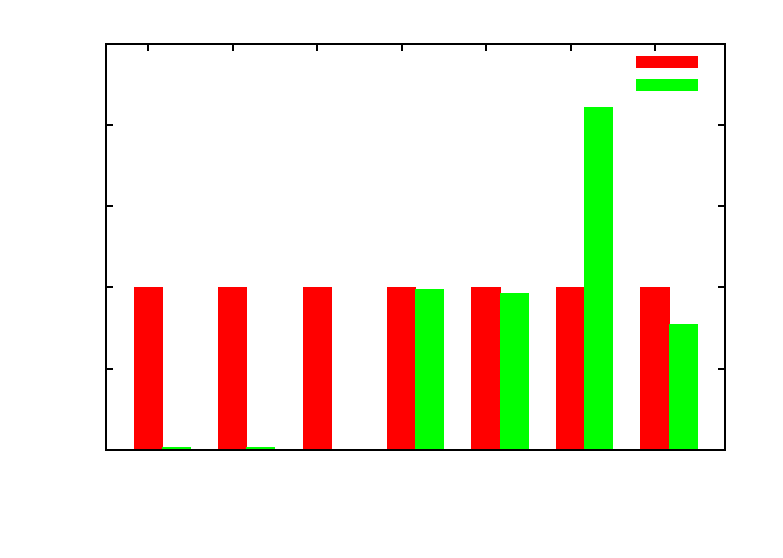
\includegraphics{popcountRankNew}}%
    \gplfronttext
  \end{picture}%
\endgroup

\end{figure}

\begin{figure}
\caption{Simple Binary Select vs. Binary Select using the Popcount instruction.}
\label{fig:selectPopcountDiff}
% GNUPLOT: LaTeX picture with Postscript
\begingroup
  \makeatletter
  \providecommand\color[2][]{%
    \GenericError{(gnuplot) \space\space\space\@spaces}{%
      Package color not loaded in conjunction with
      terminal option `colourtext'%
    }{See the gnuplot documentation for explanation.%
    }{Either use 'blacktext' in gnuplot or load the package
      color.sty in LaTeX.}%
    \renewcommand\color[2][]{}%
  }%
  \providecommand\includegraphics[2][]{%
    \GenericError{(gnuplot) \space\space\space\@spaces}{%
      Package graphicx or graphics not loaded%
    }{See the gnuplot documentation for explanation.%
    }{The gnuplot epslatex terminal needs graphicx.sty or graphics.sty.}%
    \renewcommand\includegraphics[2][]{}%
  }%
  \providecommand\rotatebox[2]{#2}%
  \@ifundefined{ifGPcolor}{%
    \newif\ifGPcolor
    \GPcolortrue
  }{}%
  \@ifundefined{ifGPblacktext}{%
    \newif\ifGPblacktext
    \GPblacktexttrue
  }{}%
  % define a \g@addto@macro without @ in the name:
  \let\gplgaddtomacro\g@addto@macro
  % define empty templates for all commands taking text:
  \gdef\gplbacktext{}%
  \gdef\gplfronttext{}%
  \makeatother
  \ifGPblacktext
    % no textcolor at all
    \def\colorrgb#1{}%
    \def\colorgray#1{}%
  \else
    % gray or color?
    \ifGPcolor
      \def\colorrgb#1{\color[rgb]{#1}}%
      \def\colorgray#1{\color[gray]{#1}}%
      \expandafter\def\csname LTw\endcsname{\color{white}}%
      \expandafter\def\csname LTb\endcsname{\color{black}}%
      \expandafter\def\csname LTa\endcsname{\color{black}}%
      \expandafter\def\csname LT0\endcsname{\color[rgb]{1,0,0}}%
      \expandafter\def\csname LT1\endcsname{\color[rgb]{0,1,0}}%
      \expandafter\def\csname LT2\endcsname{\color[rgb]{0,0,1}}%
      \expandafter\def\csname LT3\endcsname{\color[rgb]{1,0,1}}%
      \expandafter\def\csname LT4\endcsname{\color[rgb]{0,1,1}}%
      \expandafter\def\csname LT5\endcsname{\color[rgb]{1,1,0}}%
      \expandafter\def\csname LT6\endcsname{\color[rgb]{0,0,0}}%
      \expandafter\def\csname LT7\endcsname{\color[rgb]{1,0.3,0}}%
      \expandafter\def\csname LT8\endcsname{\color[rgb]{0.5,0.5,0.5}}%
    \else
      % gray
      \def\colorrgb#1{\color{black}}%
      \def\colorgray#1{\color[gray]{#1}}%
      \expandafter\def\csname LTw\endcsname{\color{white}}%
      \expandafter\def\csname LTb\endcsname{\color{black}}%
      \expandafter\def\csname LTa\endcsname{\color{black}}%
      \expandafter\def\csname LT0\endcsname{\color{black}}%
      \expandafter\def\csname LT1\endcsname{\color{black}}%
      \expandafter\def\csname LT2\endcsname{\color{black}}%
      \expandafter\def\csname LT3\endcsname{\color{black}}%
      \expandafter\def\csname LT4\endcsname{\color{black}}%
      \expandafter\def\csname LT5\endcsname{\color{black}}%
      \expandafter\def\csname LT6\endcsname{\color{black}}%
      \expandafter\def\csname LT7\endcsname{\color{black}}%
      \expandafter\def\csname LT8\endcsname{\color{black}}%
    \fi
  \fi
  \setlength{\unitlength}{0.0500bp}%
  \begin{picture}(8496.00,2590.00)%
    \gplgaddtomacro\gplbacktext{%
      \csname LTb\endcsname%
      \put(516,479){\makebox(0,0)[r]{\strut{} 0}}%
      \put(516,959){\makebox(0,0)[r]{\strut{} 50}}%
      \put(516,1438){\makebox(0,0)[r]{\strut{} 100}}%
      \put(516,1918){\makebox(0,0)[r]{\strut{} 150}}%
      \put(516,2397){\makebox(0,0)[r]{\strut{} 200}}%
      \put(1000,407){\rotatebox{-30}{\makebox(0,0)[l]{\strut{}CPU Cycles}}}%
      \put(1824,407){\rotatebox{-30}{\makebox(0,0)[l]{\strut{}Wall Time}}}%
      \put(2648,407){\rotatebox{-30}{\makebox(0,0)[l]{\strut{}BM}}}%
      \put(3472,407){\rotatebox{-30}{\makebox(0,0)[l]{\strut{}TLBM}}}%
      \put(4296,407){\rotatebox{-30}{\makebox(0,0)[l]{\strut{}L1 CM}}}%
      \put(5120,407){\rotatebox{-30}{\makebox(0,0)[l]{\strut{}L2 CM}}}%
      \put(5944,407){\rotatebox{-30}{\makebox(0,0)[l]{\strut{}L2 CHits}}}%
      \put(6768,407){\rotatebox{-30}{\makebox(0,0)[l]{\strut{}L2 CM Rate}}}%
      \put(7592,407){\rotatebox{-30}{\makebox(0,0)[l]{\strut{}L3 CM}}}%
      \put(96,1462){\rotatebox{-270}{\makebox(0,0){\strut{}Percent of Simple}}}%
    }%
    \gplgaddtomacro\gplfronttext{%
      \csname LTb\endcsname%
      \put(1668,2322){\makebox(0,0)[r]{\strut{}Simple}}%
      \csname LTb\endcsname%
      \put(1668,2202){\makebox(0,0)[r]{\strut{}Using Popcount}}%
    }%
    \gplbacktext
    \put(0,0){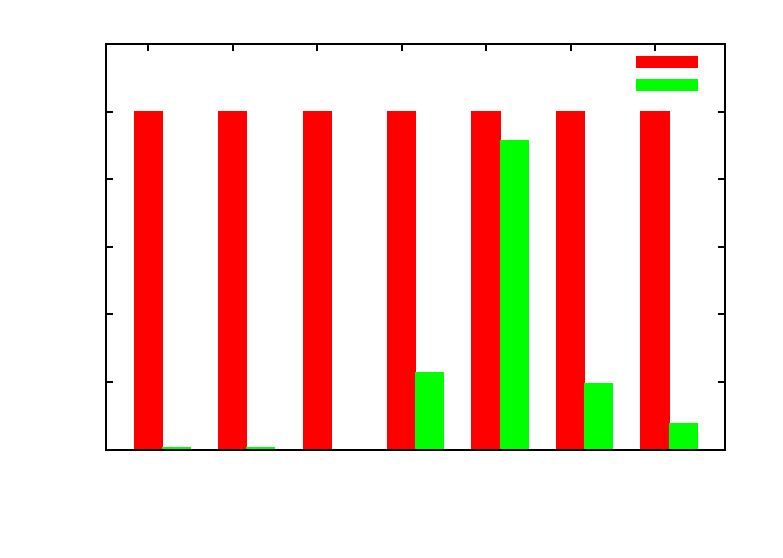
\includegraphics{popcountSelectNew}}%
    \gplfronttext
  \end{picture}%
\endgroup

\end{figure}

\begin{figure}
\caption{Values for Figure~\ref{fig:rankPopcountDiff} and \ref{fig:selectPopcountDiff}}
\label{fig:valuesForPopcountDiff}
\begin{tabular}{|l|r|r|r|}
\hline
\textbf{Rank} & no \texttt{popcount} & \texttt{popcount} & Percent \\ \hline
\textbf{CPU Cycles} & 397,345,711,110.40 & 4,423,412,635.00 & 1.113\% \\ \hline
\textbf{Wall Time} & 133,346,696.80 & 1,487,440.60 & 1.115\% \\ \hline
\textbf{BM} & 1,396,757,616.40 & 22,682.20 & 0.002\% \\ \hline
\textbf{TLBM} & 564,782.40 & 425,317.80 & 75.306\% \\ \hline
\textbf{L1 CM} & 176,090,145.60 & 175,975,752.80 & 99.935\% \\ \hline
\textbf{L2 CM} & 16,799,853.60 & 30,271,524.80 & 180.189\% \\ \hline
\textbf{L2 CHits} & 159,317,424.80 & 141,606,664.60 & 88.883\% \\ \hline
\textbf{L2 CM Rate} & 0.11 & 0.21 & 202.726\% \\ \hline
\textbf{L3 CM} & 15,935,912.60 & 10,756,189.60 & 67.497\% \\ \hline
\end{tabular}\\[5pt]
\begin{tabular}{|l|r|r|r|}
\hline
\textbf{Select} & no \texttt{popcount} & \texttt{popcount} & Percent \\ \hline
\textbf{CPU Cycles} & 1,010,898,341,664.00 & 5,223,438,088.40 & 0.517\% \\ \hline
\textbf{Wall Time} & 339,177,348.60 & 1,755,859.00 & 0.518\% \\ \hline
\textbf{BM} & 32,746,102,169.80 & 306,271.20 & 0.001\% \\ \hline
\textbf{TLBM} & 1,340,706.00 & 527,246.20 & 39.326\% \\ \hline
\textbf{L1 CM} & 128,453,042.80 & 128,173,446.40 & 99.782\% \\ \hline
\textbf{L2 CM} & 16,827,996.20 & 7,157,015.00 & 42.530\% \\ \hline
\textbf{L2 CM} & 111,653,039.00 & 120,712,813.00 & 108.114\% \\ \hline
\textbf{L2 CM Rate} & 0.15 & 0.06 & 39.338\% \\ \hline
\textbf{L3 CM} & 15,685,153.20 & 3,624,788.80 & 23.110\% \\ \hline
\end{tabular}\\[5pt]

\end{figure}

In Figure~\ref{fig:rankPopcountDiff}, \ref{fig:selectPopcountDiff}, and \ref{fig:valuesForPopcountDiff} we see the resulting relative cpu cycles, wall time, branch mispredictions, translation lookaside buffer misses, and cache misses for our rank and select queries, respectively.
We have chosen the values for the queries not using popcount to be index 100 and calculated and plotted the relative values of the queries using popcount, to show which values increase, decrease and by what relative amount, all within the same graph.
In Figure~\ref{fig:valuesForPopcountDiff} we list the actual raw values as well as the percentages graphed in Figure~\ref{fig:rankPopcountDiff} and \ref{fig:selectPopcountDiff}.

In all three figures we see that the algorithm using \texttt{popcount} is much faster, using only a fraction of the time of the other algorithm, about $0.011\%$ for rank and $0.0051\%$ for select.
We see a massive decrease in branch mispredictions both for both rank and select queries. For the select queries we see a great reduction in Translation Lookaside Buffer Misses as well as Cache Misses, especially Level 2 and 3.
For the rank queries, we see little improvement in TLBM and L1 CM, as well as a slightly larger improvement in L3 CM, but we also see a great increase in L2 CM to more than double the amount.
[TODO: speculate as to why]


The massive reduction in branch mispredictions likely accounts for some of the saved cpu cycles.
Given that the branch misprediction penalty on the Ivy Bridge architecture (on which this experiment was run) is about "15 cycles or more"~\cite{agner}, we can calculate an estimate of how many cpu cycles the branch misprediction reduction has saved us.
The number of saved branch mispredictions for \textproc{rank} is then 309,342,424.4 - 1,882.6 = 309,340,541.8 mispredictions. Assuming a penalty of 15 cycles this becomes 309,340,541.8 $\cdot$ 15 = 4,640,108,127 cpu cycles saved, and given that the total number of cycles saved is 88,918,629,772.2 - 994,895,919.6 = 87,923,733,852.6, it is 4,640,108,127 / 87,923,733,852.6 = 0.0527742388 = 5.28\% of the total amount of cpu cycles saved.
This means that the branch mispredictions do have an effect, but it is only a small part of this increase in speed. The main improvement, we expect, comes from using only a few cpu cycles per word of the bitmap to calculate the binary rank, as well as possibly the slight decrease in L1 and L3 cache misses.


By similar calculations the saved cpu cycles from branch mispredictions for \textproc{select} is at least 48,38\% of the total saved. We expect this is because of the much higher number of branch mispredictions and the lower number of cycles for the original select algorithm, as well as the fact that we can't use \texttt{popcount} for every word of the bitmap but must go back to doing manual counting of the bits when we find the word the sought-after occurrence is in.


\subsubsection{Further improvements}
Looking at the values in Figure~\ref{fig:valuesForPopcountDiff}, we find that an obvious next step would be to reduce the number of cache misses. One way to do this is to control the memory layout of the nodes and their bitmaps and then make it more likely that the queries will traverse the nodes in such a way that the next item is already in cache, either in the same cacheline or one that has been prefetched.

We will do this by placing nodes and bitmaps consecutively in memory that are mirrored pre-order in the tree, 'mirrored' meaning we go down the right side first.
We describe this in section~\ref{sec:memorylayout}.


\subsubsection{Rank and Select on naive and preallocated Tawelet Tree}

\begin{figure}
\caption{Rank and Select Running times on Wavelet Tree with increasing skew for naive construction and preallocated construction}
\label{fig:NaiveRankSkewRunningTime}
% GNUPLOT: LaTeX picture with Postscript
\begingroup
  \makeatletter
  \providecommand\color[2][]{%
    \GenericError{(gnuplot) \space\space\space\@spaces}{%
      Package color not loaded in conjunction with
      terminal option `colourtext'%
    }{See the gnuplot documentation for explanation.%
    }{Either use 'blacktext' in gnuplot or load the package
      color.sty in LaTeX.}%
    \renewcommand\color[2][]{}%
  }%
  \providecommand\includegraphics[2][]{%
    \GenericError{(gnuplot) \space\space\space\@spaces}{%
      Package graphicx or graphics not loaded%
    }{See the gnuplot documentation for explanation.%
    }{The gnuplot epslatex terminal needs graphicx.sty or graphics.sty.}%
    \renewcommand\includegraphics[2][]{}%
  }%
  \providecommand\rotatebox[2]{#2}%
  \@ifundefined{ifGPcolor}{%
    \newif\ifGPcolor
    \GPcolortrue
  }{}%
  \@ifundefined{ifGPblacktext}{%
    \newif\ifGPblacktext
    \GPblacktexttrue
  }{}%
  % define a \g@addto@macro without @ in the name:
  \let\gplgaddtomacro\g@addto@macro
  % define empty templates for all commands taking text:
  \gdef\gplbacktext{}%
  \gdef\gplfronttext{}%
  \makeatother
  \ifGPblacktext
    % no textcolor at all
    \def\colorrgb#1{}%
    \def\colorgray#1{}%
  \else
    % gray or color?
    \ifGPcolor
      \def\colorrgb#1{\color[rgb]{#1}}%
      \def\colorgray#1{\color[gray]{#1}}%
      \expandafter\def\csname LTw\endcsname{\color{white}}%
      \expandafter\def\csname LTb\endcsname{\color{black}}%
      \expandafter\def\csname LTa\endcsname{\color{black}}%
      \expandafter\def\csname LT0\endcsname{\color[rgb]{1,0,0}}%
      \expandafter\def\csname LT1\endcsname{\color[rgb]{0,1,0}}%
      \expandafter\def\csname LT2\endcsname{\color[rgb]{0,0,1}}%
      \expandafter\def\csname LT3\endcsname{\color[rgb]{1,0,1}}%
      \expandafter\def\csname LT4\endcsname{\color[rgb]{0,1,1}}%
      \expandafter\def\csname LT5\endcsname{\color[rgb]{1,1,0}}%
      \expandafter\def\csname LT6\endcsname{\color[rgb]{0,0,0}}%
      \expandafter\def\csname LT7\endcsname{\color[rgb]{1,0.3,0}}%
      \expandafter\def\csname LT8\endcsname{\color[rgb]{0.5,0.5,0.5}}%
    \else
      % gray
      \def\colorrgb#1{\color{black}}%
      \def\colorgray#1{\color[gray]{#1}}%
      \expandafter\def\csname LTw\endcsname{\color{white}}%
      \expandafter\def\csname LTb\endcsname{\color{black}}%
      \expandafter\def\csname LTa\endcsname{\color{black}}%
      \expandafter\def\csname LT0\endcsname{\color{black}}%
      \expandafter\def\csname LT1\endcsname{\color{black}}%
      \expandafter\def\csname LT2\endcsname{\color{black}}%
      \expandafter\def\csname LT3\endcsname{\color{black}}%
      \expandafter\def\csname LT4\endcsname{\color{black}}%
      \expandafter\def\csname LT5\endcsname{\color{black}}%
      \expandafter\def\csname LT6\endcsname{\color{black}}%
      \expandafter\def\csname LT7\endcsname{\color{black}}%
      \expandafter\def\csname LT8\endcsname{\color{black}}%
    \fi
  \fi
  \setlength{\unitlength}{0.0500bp}%
  \begin{picture}(4608.00,3600.00)%
    \gplgaddtomacro\gplbacktext{%
      \csname LTb\endcsname%
      \put(516,384){\makebox(0,0)[r]{\strut{} 0}}%
      \put(516,998){\makebox(0,0)[r]{\strut{} 0.5}}%
      \put(516,1612){\makebox(0,0)[r]{\strut{} 1}}%
      \put(516,2227){\makebox(0,0)[r]{\strut{} 1.5}}%
      \put(516,2841){\makebox(0,0)[r]{\strut{} 2}}%
      \put(516,3455){\makebox(0,0)[r]{\strut{} 2.5}}%
      \put(588,264){\makebox(0,0){\strut{} 2}}%
      \put(1063,264){\makebox(0,0){\strut{} 2.5}}%
      \put(1539,264){\makebox(0,0){\strut{} 3}}%
      \put(2014,264){\makebox(0,0){\strut{} 3.5}}%
      \put(2490,264){\makebox(0,0){\strut{} 4}}%
      \put(2965,264){\makebox(0,0){\strut{} 4.5}}%
      \put(3440,264){\makebox(0,0){\strut{} 5}}%
      \put(3916,264){\makebox(0,0){\strut{} 5.5}}%
      \put(4391,264){\makebox(0,0){\strut{} 6}}%
      \put(96,1919){\rotatebox{-270}{\makebox(0,0){\strut{}Wall Time (sec)}}}%
      \put(2489,84){\makebox(0,0){\strut{}Skew}}%
    }%
    \gplgaddtomacro\gplfronttext{%
      \csname LTb\endcsname%
      \put(1812,3332){\makebox(0,0)[r]{\strut{}NaiveInteger}}%
      \csname LTb\endcsname%
      \put(3459,3332){\makebox(0,0)[r]{\strut{}ControlledMemory}}%
    }%
    \gplbacktext
    \put(0,0){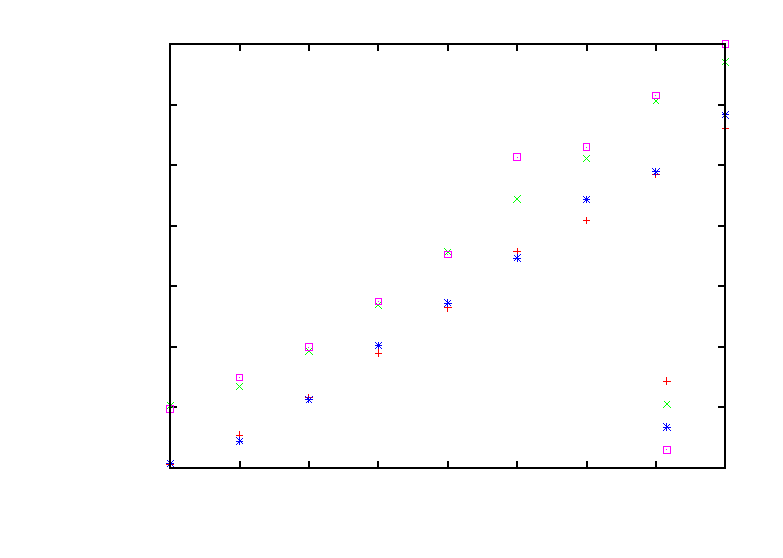
\includegraphics{naiveRankSkewRunningTime}}%
    \gplfronttext
  \end{picture}%
\endgroup

\end{figure}

